\section{Exercise 1}

Explain the design of a 1-BHT and a 2-BHT capable of executing the provided assembly code (with R0 set to 2000 and R1 set to 0).
\begin{verbnobox}[\verbarg]
LOOP:   LD F1 0 R0
        ADDD F2 F1 F1
        ADDI R1 R1 100
LOOP2:  MULTD F2 F2 F1
        SUBI R1 R1 1
        BNEZ R1 LOOP2
        SUBI R0 R0 2
        BNEZ R0 LOOP
\end{verbnobox}
Compute the number of mispredictions in the various cases. 

\subsubsection*{Solution}
The outer loop iterates $1000$ times because R0 starts at $2000$ and decreases by two each iteration.

The inner loop iterates $100$ times for each outer loop iteration because R1 starts at $100$ and decreases by one each iteration. 
Consequently, the total iterations of the inner loop amount to $1000 \times 100 = 100000$.

For the one-bit branch table computation, a finite state machine can be employed, depicted below:
\begin{figure}[H]
    \centering
    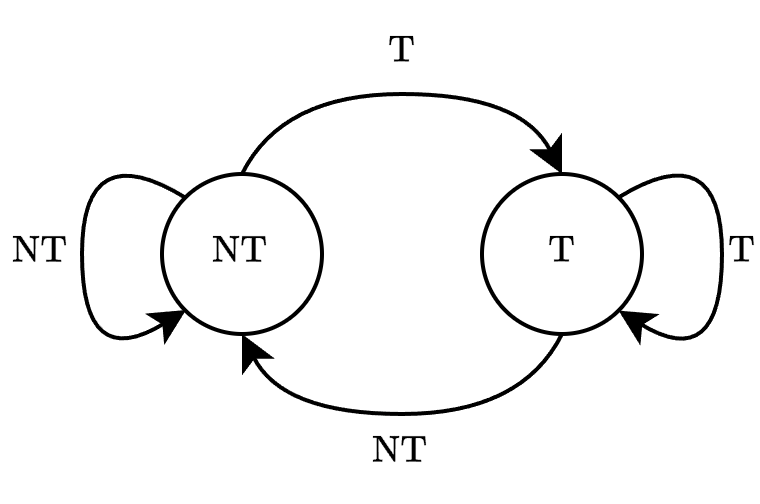
\includegraphics[width=0.4\linewidth]{images/1bht.png}
\end{figure}

In the absence of collision, one bit can be assigned for each loop. This allows four possible initializations: T-T, T-NT, NT-T, NT-NT.
\begin{itemize}
    \item For the first case (T-T), there are $1 + 1 + (1000-1) \times 2$ iterations.
    \item For the second case (T-NT), there are $1 + 1000 \times 2$ iterations.
    \item For the third case (NT-T), there are $2 + 1 + (1000-1) \times 2$ iterations.
    \item For the fourth case (NT-NT), there are $2 + 1000 \times 2$ iterations.
\end{itemize}
In the presence of collision, one bit is allocated for each loop. 
This yields two possible initializations: T, NT.
The iterations for each case are calculated as follows:
\begin{itemize}
    \item For the first case (T), there are $(1+1) \times (1000-1) + 1$ iterations.
    \item For the second case (NT), there are $1 + (1+1) \times (1000-1) + 1$ iterations.
\end{itemize}

The two-bit branch table can be designed using a finite state machine, as illustrated below:
\begin{figure}[H]
    \centering
    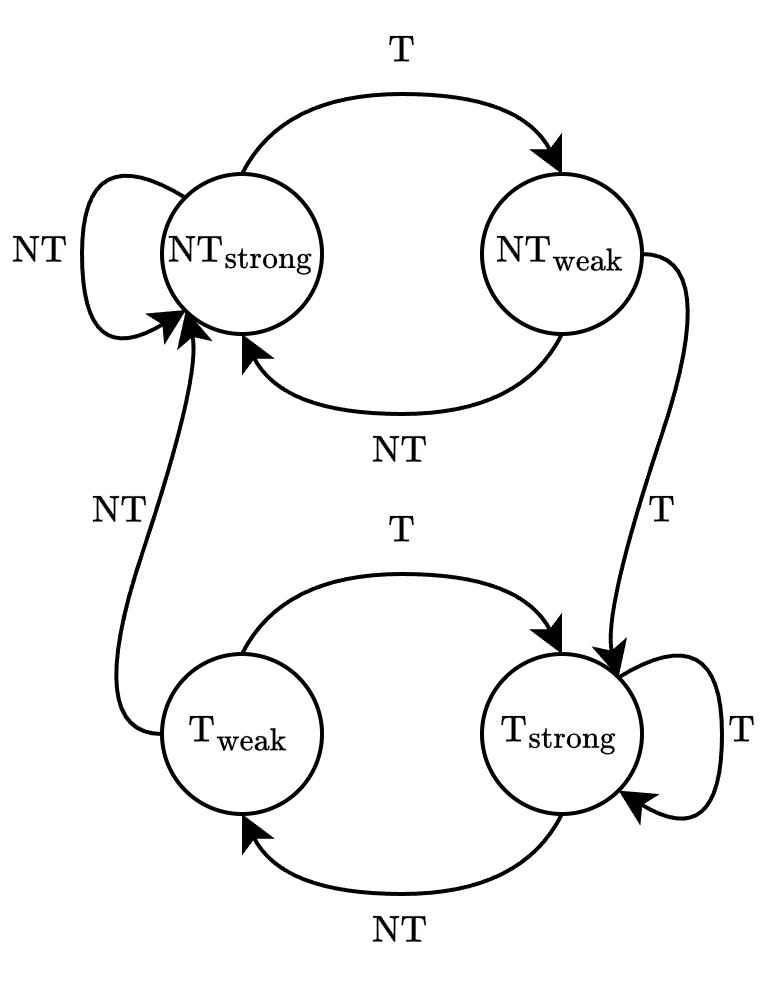
\includegraphics[width=0.4\linewidth]{images/2bht.png}
\end{figure}
In the absence of collision, where one bit is assigned for each loop, there are eight possible initializations.
The worst cases are:
\begin{itemize}
    \item $\text{NT}_{\text{weak}},\text{NT}_{\text{weak}}$: resulting in $1000 \times 2$ mispredictions for LOOP2 and $2$ mispredictions for LOOP.
    \item $\text{NT}_{\text{strong}},\text{NT}_{\text{strong}}$: resulting in $3+(1000-1)\times 1$ mispredictions for LOOP2 and $2$ mispredictions for LOOP.
\end{itemize}
The best cases are: 
\begin{itemize}
    \item $\text{T}_{\text{weak}},\text{T}_{\text{weak}}$: Resulting in $1 + (1000-1) \times 2$ mispredictions for LOOP2 and $1$ for LOOP.
    \item $\text{T}_{\text{strong}},\text{T}_{\text{strong}}$: Resulting in $1000 \times 1$ mispredictions for LOOP2 and $1$ for LOOP.
\end{itemize}

Considering these cases, the iterations for each case are calculated accordingly:
\begin{itemize}
    \item For the first case, we have $1 + 1 + (1000-1) \times 2$.
    \item For the second case, we have $1 +1000 \times 2$.
    \item For the third case, we have $2 + 1 + (1000-1) \times 2$.
    \item For the fourth case, we have $2 +1000 \times 2$.
\end{itemize}

In the presence of collision, where one bit is used for each loop, there are four possible initializations ($\text{T}_{\text{strong}}$, $\text{T}_{\text{weak}}$, $\text{TN}{\text{strong}}$, $\text{NT}:{\text{weak}}$). 
The iterations for each case are calculated as follows:
\begin{itemize}
    \item For the first case, we have $1 \times 1000 + 1$.
    \item For the second case, we have $1 \times 1000 + 1$.
    \item For the third case, we have $2 + 1 \times 1000 + 1$.
    \item For the fourth case, we have $1 + 1 \times 1000 + 1$.
\end{itemize}

Comparing the worst-case scenario of the two-bit branch table with the best-case scenario of the one-bit branch table, it's evident that the worst 2BHT performs better than the best 1BHT.